\documentclass[12pt,a4paper]{article}

\usepackage{ctex}
\usepackage{amsmath, amssymb, physics,mathrsfs,ntheorem}
\usepackage{titlesec}
\usepackage[left=3.17cm, right=3.17cm, top=2.54cm, bottom=2.54cm, bindingoffset=0cm, headheight=1.5cm, footskip=1.75cm]{geometry}
\usepackage{fancyhdr}
\usepackage{tikz}
\usepackage{booktabs}
% \usepackage[hidelinks]{hyperref}
\usepackage{hyperref}
\usepackage{cite}
\usepackage{cases}
\usepackage[ruled,linesnumbered]{algorithm2e}
\usepackage{graphicx} %use graph format
\usepackage{epstopdf}
\usepackage{siunitx}
\usepackage{subcaption}
\usepackage{caption}
\usepackage{pdfpages}
\usepackage{listings}
\usepackage{enumitem}
\usepackage{titletoc}
\usepackage{shadowtext}      % 阴影效果
\usepackage{stackengine} % 用于自定义下划线的宏包
\usepackage{setspace}
\usepackage{tocloft} % 包含对目录和标题的自定义支持

% 修改 "图像表" 的标题为 "本文图像"
\renewcommand{\listfigurename}{本文图像}
% 修改 "表格目录" 的标题为 "本文表格"
\renewcommand{\listtablename}{本文表格}

% 让标题左对齐
\renewcommand{\cftloftitlefont}{\raggedright\large\bfseries} % 图像标题
\renewcommand{\cftlottitlefont}{\raggedright\large\bfseries} % 表格标题


% 在图号前加上“图”
\renewcommand{\cftfigpresnum}{图 }
% 在表号前加上“表”
\renewcommand{\cfttabpresnum}{表 }

% 增加编号与标题之间的间隔,避免文字重叠
\setlength{\cftfignumwidth}{3em} % 图像序号宽度
\setlength{\cfttabnumwidth}{3em} % 表格序号宽度


\setstackgap{L}{1.0mm}  % 调整下划线与文本之间的距离

\renewcommand{\contentsname}{目\quad 录}
\titlecontents{section}
  [0em] % 左边距
  {\contentslabel{0em}} % 代码块
  {\hspace*{1em}} % 代码块
  {} % 代码块
  {\titlerule*[0.6pc]{$.$}\contentspage} % 格式

\titlecontents{subsection}
  [1.5em] % 左边距
  {\contentslabel{0em}} % 代码块
  {\hspace*{1.5em}} % 代码块
  {} % 代码块
  {\titlerule*[0.6pc]{$.$}\contentspage} % 格式


\renewcommand{\lstlistingname}{本文代码}

\lstset{
    basicstyle          =   \sffamily,          % 基本代码风格
    keywordstyle        =   \bfseries,          % 关键字风格
    commentstyle        =   \rmfamily\itshape,  % 注释的风格,斜体
    stringstyle         =   \ttfamily,  % 字符串风格
    flexiblecolumns,                % 别问为什么,加上这个
    numbers             =   left,   % 行号的位置在左边
    showspaces          =   false,  % 是否显示空格,显示了有点乱,所以不现实了
    numberstyle         =   \zihao{-5}\ttfamily,    % 行号的样式,小五号,tt等宽字体
    showstringspaces    =   false,
    captionpos          =   t,      % 这段代码的名字所呈现的位置,t指的是top上面
    frame               =   lrtb,   % 显示边框
}

\lstdefinestyle{Python}{
    language        =   Python, % 语言选Python
    basicstyle      =   \zihao{-5}\ttfamily,
    numberstyle     =   \zihao{-5}\ttfamily,
    keywordstyle    =   \color{blue},
    keywordstyle    =   [2] \color{teal},
    stringstyle     =   \color{magenta},
    commentstyle    =   \color{red}\ttfamily,
    breaklines      =   true,   % 自动换行,建议不要写太长的行
    columns         =   fixed,  % 如果不加这一句,字间距就不固定,很丑,必须加
    basewidth       =   0.5em,
}



\bibliographystyle{siam}

\captionsetup{
    font={small,stretch=1},
    singlelinecheck=true
}

\renewcommand{\arraystretch}{1.2}  % 1.5倍行距

\pagestyle{fancy}
\fancyhead{}
\fancyfoot{}
\fancyfoot[C]{\thepage}
\renewcommand{\headrulewidth}{0pt}
\renewcommand{\footrulewidth}{0pt}
\renewcommand{\abstractname}{\large{摘要}} %更改摘要二字的样式

\setCJKmainfont{宋体-简} % 设置字体为宋体
\setmainfont{Times New Roman} % 设置英文字体为Times New Roman
\linespread{1}% 设置行距

% 定义黑体字体 (Mac上可以使用STHeiti或SimHei)
\setCJKfamilyfont{heiti}{黑体}
% 自定义黑体的命令
\renewcommand{\heiti}{\CJKfamily{heiti}}
\setCJKfamilyfont{huawenxinwei}{华文新魏}
\newcommand{\huawenxinwei}{\CJKfamily{huawenxinwei}}
\setCJKfamilyfont{lishu}{报隶-简}
\renewcommand{\lishu}{\CJKfamily{lishu}}

\titleformat{\section}{\fontsize{14pt}{14pt}\heiti\bfseries\centering}{\thesection}{0.5em}{}
\titleformat{\subsection}{\fontsize{12pt}{12pt}\bfseries}{\thesubsection}{0.5em}{}
\titleformat{\subsubsection}{\fontsize{12pt}{12pt}\bfseries}{\thesubsubsection}{0.5em}{}


% \newtheorem{theorem}{定理}
% \newtheorem{lemma}{引理}
\newtheorem*{lemma}{引理}
% \newtheorem{assumption}{假设}

% 伪代码算法格式
\renewcommand{\algorithmcfname}{算法}
\renewcommand{\thealgocf}{}
\SetKwInput{KwIn}{输入}
\SetKwInput{KwOut}{输出}
\SetKwRepeat{Do}{do}{while}
\SetAlgoCaptionSeparator{: } %伪代码分隔符表头



\def\mytitle{数学建模论文题目}
\title{\mytitle}
\date{}



\begin{document}

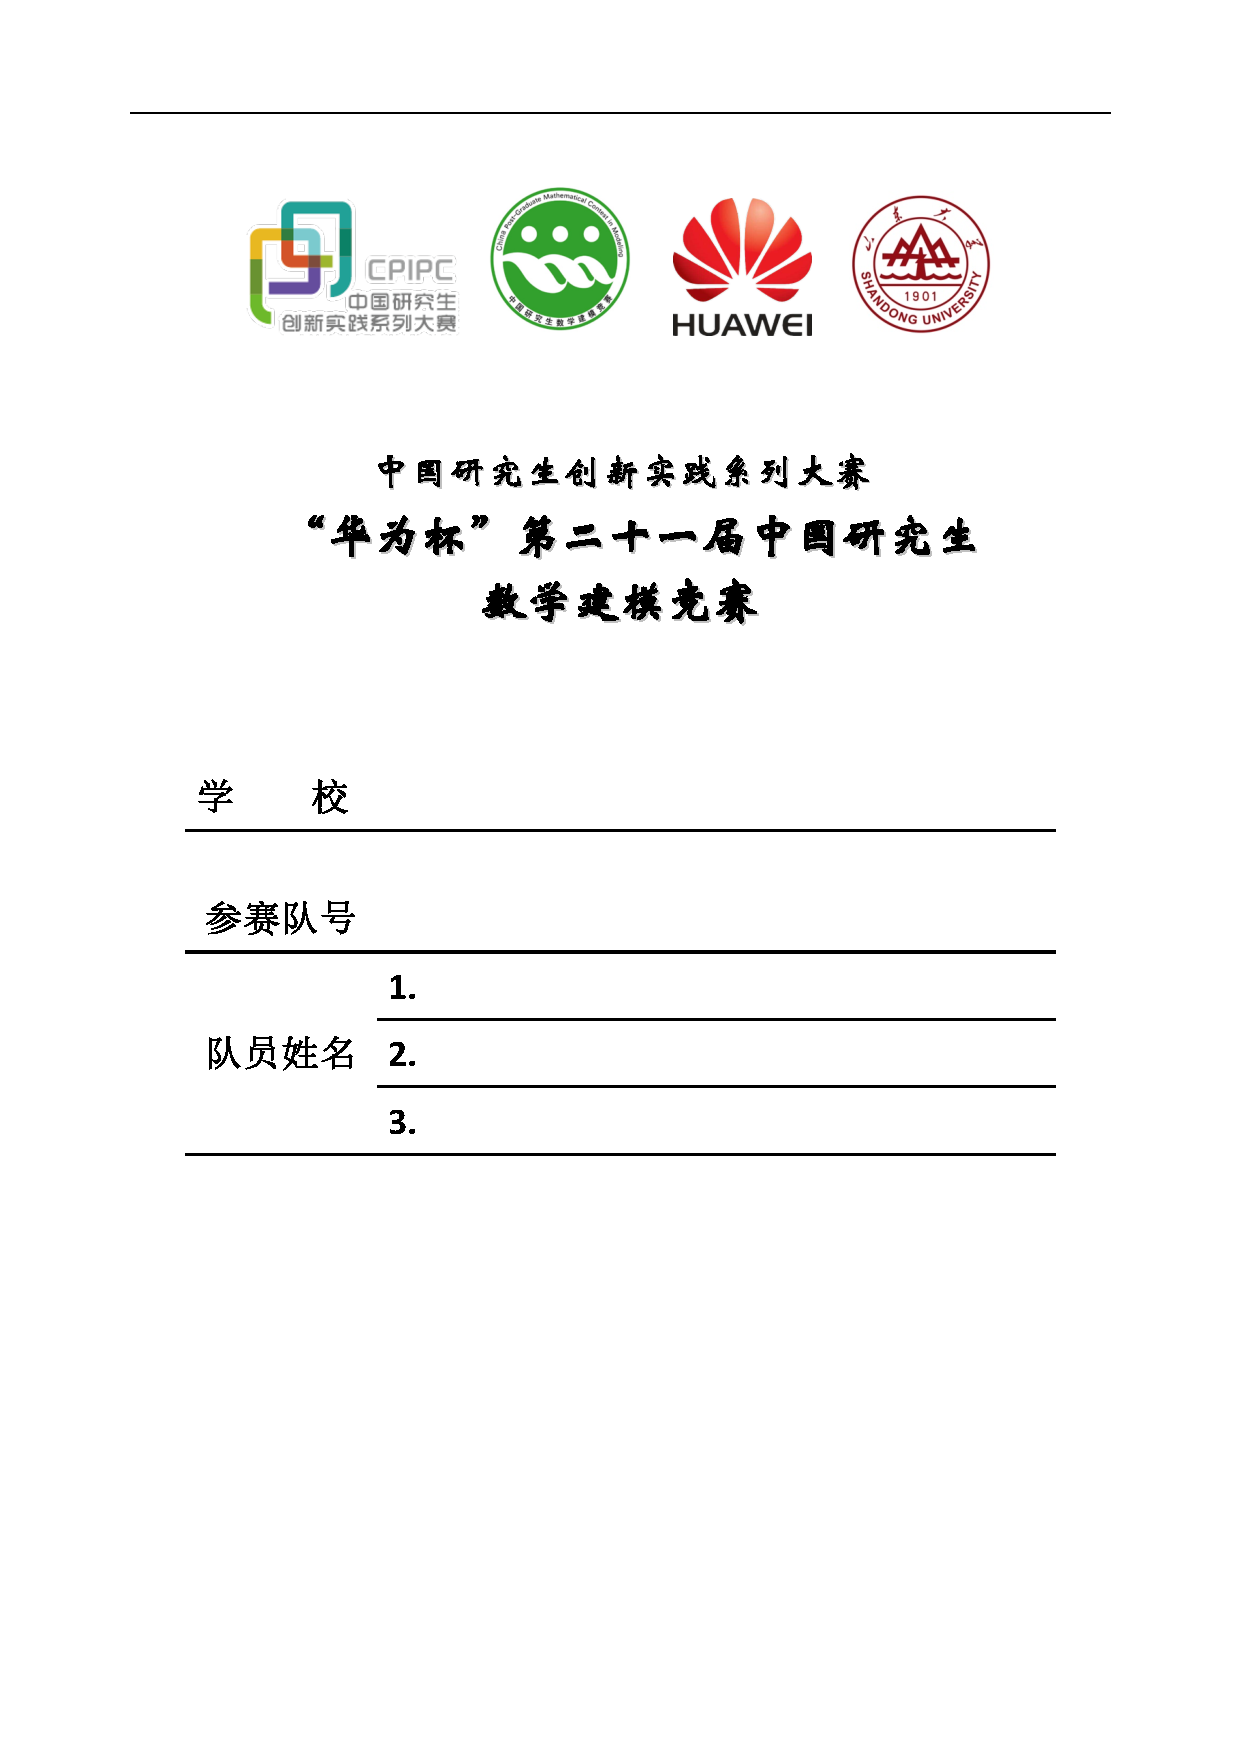
\includepdf[pages=-]{src/封面.pdf}

\clearpage
\thispagestyle{empty} 
\vspace*{1em}
\begin{center}
    \fontsize{18pt}{18pt}\selectfont % 小二号字体
    \huawenxinwei % 使用华文新魏字体
    \shadowtext{\textbf{中国研究生创新实践系列大赛}}
\end{center}
\begin{center}
    \fontsize{22pt}{22pt}\selectfont
    \huawenxinwei % 使用华文新魏字体
    % \shadowoffsetx{-12pt}
    \shadowtext{\textbf{ “华为杯”第二十一届中国研究生}}
\end{center}
\begin{center}
    \fontsize{22pt}{22pt}\selectfont
    \huawenxinwei % 使用华文新魏字体
    \shadowtext{\textbf{数学建模竞赛}}
\end{center}

\vspace*{1em}

\begin{center}
题目\stackunder{\fontsize{16pt}{16pt}\selectfont\heiti\textbf{\mytitle}}{\rule{\widthof{\fontsize{16pt}{16pt}\selectfont\heiti\textbf{\mytitle}+1}}{0.4pt}}
\end{center}


\begin{center}
    \large\textbf{摘要}
\end{center}
在这里书写摘要

\vspace*{1em}

\textbf{\large{关键词:}}
关键词1; 关键词2; 关键词3

\clearpage
% 目录页
\pagenumbering{gobble}
\tableofcontents

\clearpage
\pagenumbering{gobble}
% 图像表格目录
\listoffigures 


\vspace*{4em}

\listoftables



\clearpage
\pagenumbering{arabic}
\setcounter{page}{1}


\clearpage
\section{问题重述}
\subsection{问题背景}





\subsection{问题描述}

本文需要解决如下问题:

\begin{enumerate}[label=\hfill\arabic*.,left=0pt]
    \item XXXXXXX;
    \item XXXXXXX;
    \item XXXXXXX;
\end{enumerate}

\clearpage
\section{模型假设与符号说明}
\subsection{模型假设}

在建立模型时,需要考虑以下假设:
\begin{enumerate}[label=\textbf{假设} \arabic*,left=0pt,itemsep=0pt]
    \item XXXXXXX;
    \item XXXXXXX;
    \item XXXXXXX;
    \item XXXXXXX;
    \item XXXXXXX;
\end{enumerate}


\subsection{符号说明}

\begin{table}[h!]
    \centering
    \caption{符号说明}
    \begin{tabular}{cl}
    \toprule
    符号 & 含义  \\ 
    \midrule
    $A$ & XXXXX  \\
    \bottomrule
    \end{tabular}
    \label{table:符号说明}
    \end{table}

    \clearpage
\section{问题分析与求解思路}
\subsection{问题分析}
(一)问题一的分析

XXXXXXXXX

(二)问题二的分析

XXXXXXXXX

(三)问题三的分析

XXXXXXXXX

(四)问题四的分析

XXXXXXXXX

\subsection{求解思路}

\begin{figure}[htbp]
    \centering
    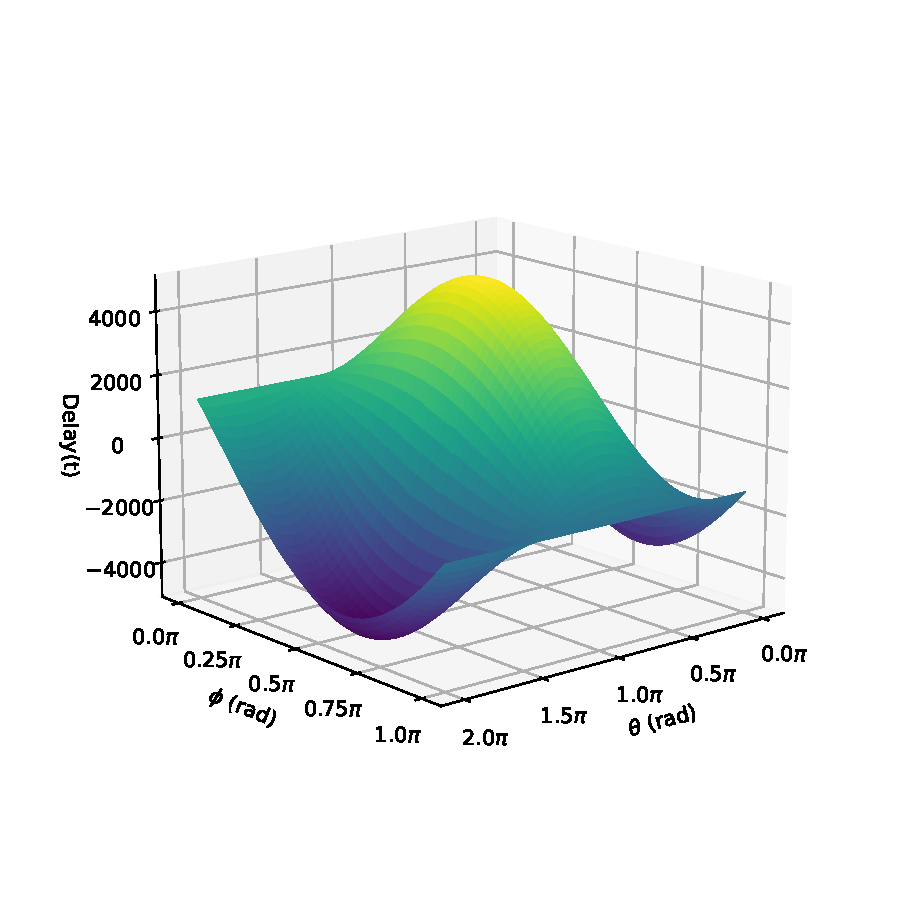
\includegraphics[width=0.9\linewidth,trim=20 50 0 50, clip]{src/Geo_3d.pdf}
    \caption{求解思路示意图}
    \label{fig:求解思路}
\end{figure}


\clearpage
\section{问题一的模型建立与求解}
\subsection{问题一的模型建立}


\subsection{问题一的模型结果}\label{问题一的模型结果}


\begin{algorithm}
    \caption{不动点迭代法}\label{不动点迭代法}
    \KwIn{给定迭代函数$g(x)$、初始估计$\tau^{(0)}$、最大迭代次数$N$、收敛准则$\epsilon$}

    \KwOut{迭代$\tau^*$}

    \For{$n < N$}{
        计算$\tau^{(n+1)} = g(\tau^{(n)})$

        \If{$|\tau^{(n+1)} - \tau^{(n)}| < \epsilon$}{
            退出迭代循环
        }
    }
\end{algorithm}



\begin{table}[h!]
    \centering
    \caption{表格题注}
    \begin{tabular}{cc|cc}
    \toprule
    参数 & 值 & 参数 & 值 \\ 
    \midrule
    1 & 2 & 3 & 4 \\
    \bottomrule
    \end{tabular}
    \label{table:表格题注}
    \end{table}

参考\cite{key},XXXXXXXX。

\clearpage
\section{问题二的模型建立与求解}\label{问题二的模型建立与求解}

\subsection{模型构造}

\subsection{模型求解}

\clearpage
\section{问题三的模型建立与求解}

\subsection{模型构造}

\subsection{模型求解}

\clearpage
\section{问题四的模型建立与求解}

\clearpage
\section{总结与评价}
\subsection{优点}



\subsection{缺点}

\subsection{展望}




\clearpage
% \section*{参考文献}
\addcontentsline{toc}{section}{参考文献}
% \bibliography{cite.bib}
\begin{thebibliography}{99}
    \bibitem{key} 引用信息
    

\end{thebibliography}

\clearpage

\section*{附录}
\addcontentsline{toc}{section}{附录}
\phantomsection 

\lstinputlisting[
    style       =   Python,
    caption     =   {\bf HelloWorld.py},
    label       =   {HelloWorld.py}
]{src/code/HelloWorld.py}



\end{document}